There are several types of low-level task the surgeon usually employs while
performing the surgery.
%
\christian{One common procedure is reconnection and joining of blood vessels. [should be put on the following list...]}.
Another is fixing the stenosis of aorta where the three most common types of fixing
the problem are:

\begin{description}

  \item[End to end aortoplasty:] the surgeon completely cuts away the
    affected part of aorta and sutures the two ends of aorta back together.

  \item[Patch aortoplasty:] the surgeon performs a cut along the axis of
    the aorta thus allowing the narrow place to expand. Then applies a
    patch from artificial material to fill the hole in.

  \item[Subclavian flap aortoplasty:] the nearest artery is cut,
    removing also half of the artery (along the axis) and part of the
    aorta in the affected place. He then uses the rest of the artery to
    patch the aorta.

\end{description}

\christian{Insist that our method is able to simulate all these surgical tasks}
From our point of view all these procedures share the same similarity:
Parts of the circulatory system are sutured together or to a patch. 
\christian{These parts are not too far away from each other. (?)} 
On this we have based our general approach in the simulation. 
The simple way how to perform the suturing would be to connect the respective edges with springs. 
This approach however adds some unwanted energy to the system. 
Our method is based solely on the relaxation of the mesh of shell elements.
%% christian: I like the "relaxation" term !!!

We start with a mesh representing the situation after all the cuts have been performed but before suturing takes place. 
\christian{I think that we should precise that we do not simulate suture : We are working on a planning system not a training simulator, and a trained surgeon knows how to perform the sutures.}
In the first step we select on the mesh edges that we want to suture together and join the corresponding nodes together. 
\christian{The result is topologicaly different mesh that has same number of elements. (not clear)}
The Figure \ref{fig-JoiningVessels} explains this operation when joining vessels. 
Then we start the simulation on the modified mesh while using the original mesh to define rest shapes of some shell elements. 
\christian{ \sout{After the mesh relaxes and the simulation reaches energetical equilibrium the simulation terminates.}
We progressively recontract the rest shape of the relaxed shells to their initial shapes. 
The energetical equilibrium found by the simulation gradually forces the side edges to connect.}

\begin{figure}[tbh]
\begin{center}
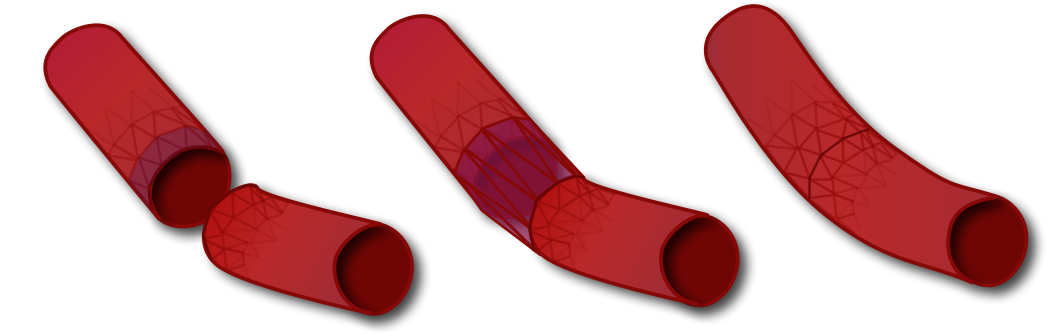
\includegraphics[width=\columnwidth]{img/rest_shape_scheme.png}
\end{center}

\caption{Scheme showing the method for joining two vessels. \christian{Do we need to extend the scheme for every type of aortoplasty (end to end / Patch / Subclavian): it would illustrate that the relaxation method works for every case...} }
\label{fig-JoiningVessels}
\end{figure}

If the nodes that are to be sutured together are not in a close vicinity we may experience unwanted quick increase of internal forces at the beginning of the simulation.
To allevieate this problem we have implemented the technique that allows for moderate changes in the rest shape between simulation steps.
\christian{Between the start and the end of the simulation we use a linear interpolation of the rest shape for the shells that are relaxed}
\christian{\sout{At the start of the simulation we use different rest shape mesh.}}
\christian{I think that it is unclear that we do the relaxation on some shells that are on the side edges of the connecting line}
It is topologicaly equivalent to the original mesh but nodes have positions equivalent to the simulated mesh (that way the initial deformations are not so big) \christian{unclear...should be illustrated ?}. 
\christian{\sout{During the simulation we then perform several steps of linear interpolation between these two rest shape meshes. }}
At the end of interpolation the original rest shape is used. 
After the mesh relaxes the simulation again terminates.

% vim: et sw=2 tw=75 fdm=marker fdc=2 spell
